\chapter{Market Analysis}
	In the course CCM, the group had to make a market analysis which
   investigates the possibilities of selling the software on the global
   market. To find out if it is viable and how to go about it. A study
    on a fictional company, that the group made up, was done and also a
     study of a chosen market’s culture was done for the use to potentially
      further development of our software.
	\\
	\section{Going international or not?}
	Reasons for going international:
	\begin{itemize}
		\item Bigger Market
		\begin{itemize}
			\item Thanks to the fact that our product is developed in an
       international language, it is accessible for a broad audience
		\end{itemize}
		\item Bigger Audience
		\begin{itemize}
			\item A simple fact is that there are not many big game development
       companies in our little country. So if we want to become a part of
        a bigger company, we will need to get seen by as many as possible
		\end{itemize}
	\end{itemize}
	Reason not to go international:
	\begin{itemize}
		\item Difference in cultures may cause conflicts/disagreements
		\begin{itemize}
			\item Different countries may have different views on what a good game
       looks like. If we should choose to distribute to a country that
        dislikes our product, the country may give us a bad image based
         on their views
		\end{itemize}
	\end{itemize}
	\begin{itemize}
		\item Need for bigger hardware specs
			\begin{itemize}
				\item If we distribute our game for a bigger market, the hardware
         specs will need to be higher as there will be more users and
          longer between the player
			\end{itemize}
	\end{itemize}
	\begin{itemize}
		\item Need for broader company staff across countries
	\end{itemize}
	\begin{itemize}
	\item 	If we would go international there’s a high possibility the resources
   needed to maintain the company will exceed our current staff’s limits.
    Therefore, we would have to hire staff in different countries, which
    can be both good and bad. The bad thing could be that it would make
    it more difficult or complicated to maintain an overview of the company
     and the progress altogether. And eventual conflicts will be difficult
     to appropriately handle.
		 \end{itemize}
	\\
	\section{SWOT Analysis}
	In here we look at our fictional company’s goals and strengths, and how
   our product will fare on the market.
	\\
	\subsection{Mission and Goals}
	Our small game company, Small Dinghy Software, consist of six students
   and is focused and determined to make a game for the international market,
    and to make a profit from the sales of the game. We don’t plan to make a
     living of the sales, only to make a profit. The focus will be on the
     western market, but will still be accessible on a global scale. This
     will be done using the Steam platform from Valve Corporation, which
     in turn will be a huge benefit for future customers and handling of
     taxation.
	\\
	\subsection{Eternal Environment}
	\textbf{Legal protection and rights}
	\\
	Our game Shipwars Online, which is based on the classic board game
   “Battleships”, could not use that name, since it was licensed by the
   company who made the movie “Battleships”. This was the reason for naming
    the game Shipwars Online instead. We could in turn license the name
     “Shipwars” as a franchise, to ensure that our game will not be mistaken
      for another game with the same name.
	\\
	\\
	\textbf{Trade restrictions}
	\\
	Since we currently only plan to use the Steam platform as our sales
  platform, we will be limited to the users of Steam as our potential
  customers, which is not a bad thing, since Steam has a huge user/customer
  base of approximately 6 million people online on the service every day.
	\\
	\begin{figure}[h]
	\centerline{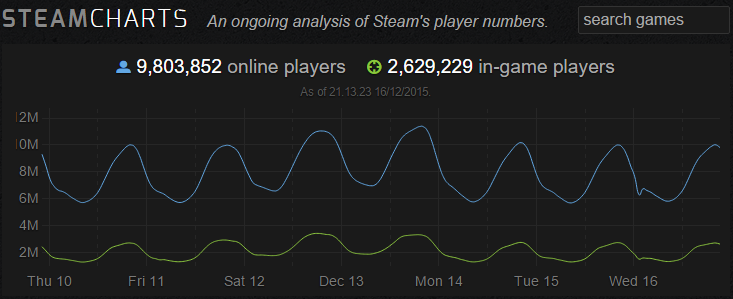
\includegraphics[scale=0.63]{SteamCharts}}
	\caption{Steam chart of users playing}
	\end{figure}
	\\
	\textbf{Shifting Production \& Consumption}
	\\
	Competing software products emerging on Steam can change the balance of
   consumption and sale of Shipwars Online. Clones could emerge that try to
    take a share of the market. Sales on Steam can push more people to buy
    the product if wanted by the developer. In terms of production, it is
    basically nothing, as the product only exists as an intangible virtual
     product.
	\\
	\\
	\textbf{Strengths}
	The strengths in our company is the game itself. With an internationally
  known game that has a similar style as the original board game
  “Battleships”, we hope that the memory of the board game will attract
  the players to our online game. The game will be bought for a one-time
   fee, and after be free for the user to play. Our company focuses on
    keeping the game interesting and fun for the gamers around the world.
     With the skilled employees, we aim to keep the game professional and
     up to date.
The highest cost in our firm will be the server maintenance, that have to
withstand the pressure of a high amount of players.
	\\
	\\
	\textbf{Weaknesses}
	The marketing for our company is low budget. As we are a new player
  on the market, we need to keep cost down, but also distribute our game
   out to the public. Therefore, online advertisement on different sites
    are what we can afford for now. The competitions are the board game
     itself, and as it stands we have the upper hand, that is mostly because
     of the growing industry online, where the board games are beginning to
     lose market share. On the technical front we are not the most developed.
	\\
	\\
	\textbf{Opportunities}
	The game is online and therefore it fits with the emerging trends of online
   games. Access to an international market allows a potential large
    player-base growth if the marketing and choice of platform is just right.
	\\
	\\
	\textbf{Threats}
	Most of the threats to our product comes from the fact that our company
   is not big, so we don’t have access to a big security network. An example
   would be that we don’t have much claim on our game in terms of copyright
   and access to lawyers if someone violates it.  Also we have to consider
    the copyrights of the company who first developed the “Battleship” board
     game and make sure we have an agreement with them before releasing our
     online version.
	\\
	\\
	As the company’s products focus on software the international market would
   be the ideal candidate. Software can be deployed across most of the world,
    as it can be distributed wirelessly and wired through the Internet.
    Software can be targeted to any specific country if needed, since the
    code is not set in stone.
	\\
	\section{Strategy for going international}
	Entering an overseas market in relation to Denmark requires looking into
   physical and virtual platforms situated in these locations. Physical
    platforms allow software to be resold through export to various
     brick-and-mortar businesses around the world. Virtual platforms allow
      software to be sold through either third-party licensing or through
       direct sales in a home-brewed platform.
	\\
	\\
	In America, the virtual platform Steam is available as a software
   distributor, mostly focusing on games. Steam allows a software
   organisation to deploy and sell their software requiring no exclusivity.
    What Steam gets from this deal is a cut on the sale. Steam only applies
     to desktop (Windows, OSX, Linux), so other platforms would be needed in
      order to supplement other directions such as mobile
      apps (eg. App Store and Google Play Store).
	\\
	\\
	The company chose the licensing strategy. This was done because it would
   let the company keep control and ownership of the product. It also opens
    up for the possibility that the company can expand the product to other
     international markets. Another reason to keep control of the game is so
      that the company can improve and expand the game.
	\\
	\\
	Licensing also allows a small, if not non-existent, transport cost. Any
   transport cost would be with network bandwidth. However, with a third-party
    licensing platform, such as Steam, this cost is shifted onto the
     platform owner, instead of the developer.
	\\
	\\
	The company chose the Steam platform because Steam offer a lot of help
   to small companies and individual developers who wish to release games
    but does not know the intricacies of licensing policy.
	\\
	\\
	We have also tried to check if different cultures would react differently
   to our game. There was not much information on the subject, other than
   some countries can ban your game if they find it offensive. Because our
   game is a remake of the old board game, the likelihood of the game being
    banned is minimal. Also the age group for our customers, would most
    likely be in the age regime of nearly all ages. This is again because
     it is a board game, and can be played with everybody as soon you know
     the rules to the game, and it will be fairly simple to play.
